\subsection{Cluster tests}\label{sec:clustertest}
In this section we perform a number of tests on a cluster setup described in \Cref{sec:clustersetup}. The cluster setup is important due to the large size of data used for these tests.
We use a 2/3 split on all of our data, yielding 1348428 games for training and 577552 for testing.
\subsubsection{Feature tests}\label{sec:feattest}
A number of tests are performed to see if combining different types of features may be beneficial.
Tests are performed using logistic regression using stochastic gradient descent and L2 regularisation with a ridge value of 0.01. 
For each feature test 1348428 games are used for training and 577552 games are used for evaluation. 
The different types of features tested are:
\begin{enumerate}
\item $\phi_\text{SINGLE}$
\item $\phi_\text{PAIR}$
\item $\phi_\text{SINGLE}$, $\phi_\text{PAIR}$
\item $\phi_\text{SINGLE}$, $\phi_\text{PAIR}$, $\phi_\text{COUNTER}$
\item $\phi_\text{SINGLE}$, $\phi_\text{PAIR}$, $\phi_\text{COUNTER}$, $\phi_\text{BEST-RANK}$
\end{enumerate}

\begin{figure}[!htb]
  \centering
  % Graph for feature tests. 
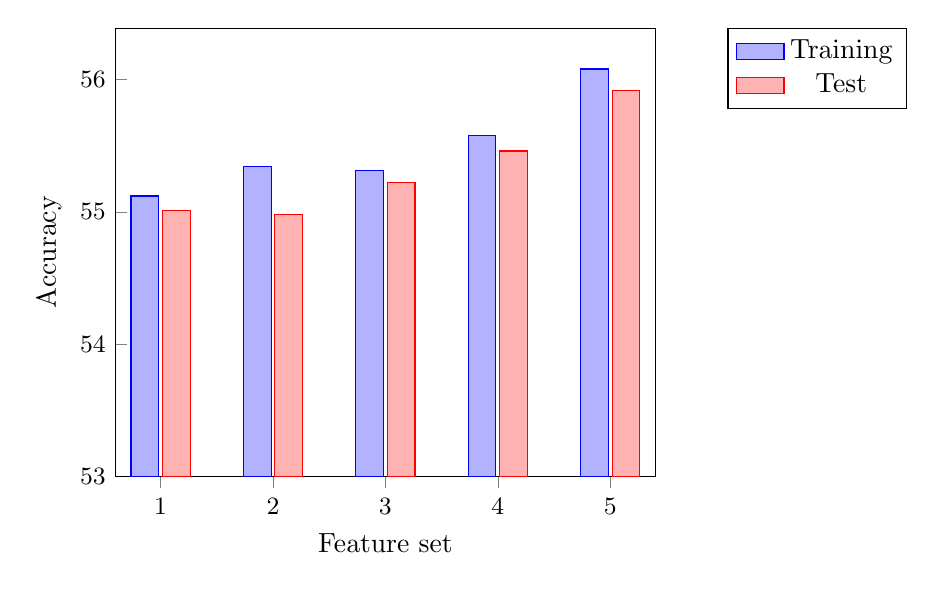
\begin{tikzpicture}
\begin{axis}[
    ybar,
    ylabel = Accuracy,
    xlabel = Feature set,
    tick label style={font=\small},
    tickpos=left,
    xticklabels={1, 2, 3, 4, 5}, 
    xtick={1,2,3,4,5},
    ymin=53,
    legend entries={Training,Test},
    legend style={at={(1.3,1.0)},
        anchor=north,legend columns=1
    },
    legend image code/.code={%
      \draw[#1] (0cm,-0.1cm) rectangle (0.6cm,0.1cm);
    }   
    ]   
    \addplot +[bar shift=-.2cm] coordinates {(1,55.12) (2,55.34) (3,55.31)  (4,55.58)     (5,56.08)};

    \addplot  +[bar shift=.2cm]coordinates {(1,55.01) (2,54.98) (3,55.22) (4,  55.46) (5,55.92)};

\end{axis}
\end{tikzpicture}
   \caption{Accuracy of features}\label{fig:cluster-feat}
\end{figure}

The feature evaluation results from \Cref{fig:cluster-feat} shows two interesting results, by looking at each individual test case we see the we have almost no overfitting. The largest difference is data point 2: (pairs) with a difference of $3.610^{-3}$ percentage points. The results shows some tendency between the complexity of the model and the performance of the classifier. Higher complexity in general yields a better classifier. The best result was achieved using all pre-match features.




